For a real world recognition task, an algorithm that can continuously adaptive to new labels just like the human does, is always very attractive and practical.
In this section, we propose a method for online adaptive learning with a few labeled data in both domain and target examples using the features extracted from GoogLeNet. We design the following experiment, transferring from Food-101 dataset to Food-256 dataset to illustrate our method while just using a few examples. Since Food-101 has more images per category, we use it as the source domain and the fine-tuned GoogLeNet on Food-101 from Section \ref{sec:ft} is used as the feature extractor to generate feature representations for both datasets. The Food-101 and Food-256 datasets share about 46 categories of food even though the images in the same category may vary across these two datasets. The types of food in Food-101 are mainly western style while most types of food in Food-256 are typical Asian foods. To make this task more challenging, we also limited the number of examples in both source and target domain. Unlike those previous studies which only consider the performance within the target domain, since the two domains are within the general food domain, we also consider how our method performs on the target domain incorporating the source domain. The experiment results show that not only can our method adapt the new categories, but also it can keep a relatively high overall accuracy for both source and target domains.
For the rest part of this section, we first discuss the limitation of some previous domain adaptation approaches for our task, then we introduce our method and show the improved performance on the same task.
\subsection{Limits of previous approaches}
From previous studies, there are two kinds of approach to solve our task. The first approach is to fine-tuning the deep CNN with the target examples incorporating with the sources ones.
Fine-tuning the deep CNN model focuses on learning good feature representations from the images and using linear models for classification. From Section \ref{sec:ft}, we successfully use this approach to transfer the knowledge from a general domain to our food domain with impressive results. Indeed, deep CNN can learn discriminative features and by taking advantage of this, this approach achieved some impressive results from previous studies\cite{Chatfield14} \cite{zeiler2014visualizing}. However, fine-tuning on deep CNN requires an ample amount of labeled target data and sometimes could degrade the performance when the labeled examples are scarce\cite{hoffman2013one}. There are many hyperparameters that affect the performance of deep CNN and fine-tuning it on a sparse label condition can lead to horrible overfitting. Apart from its sensitivity to the hyperparameters, fine-tuning the whole network requires intensive computational resources which makes it inappropriate for online learning.

Rather than learning efficient representations, another typical approach are more focused on dealing with the representation learned from conventional feature extraction methods for domain adaptation.
%Many methods have been proposed by minimizing the representation distance between the source and target domain in an unsupervised manner \cite{gong2012geodesic}\cite{fernando2013unsupervised}.
Supervised domain adaptation models, such as Adaptive-SVM (A-SVM) and PMT-SVM, try to utilize the knowledge from source domain and apply to target domain\cite{yang2007adapting}\cite{aytar2011tabula}. These methods are limited in our task for the following reasons: all these methods try to find the similarity between the source and target domain. Indeed, they show some good performance when these two domains have many overlapped or similar categories. From empirical experiments, we find that they suffer when the target domain is different from the source one. Table \ref{tab:su_domian} shows some empirical experiment results for two typical domain adaptation methods in a binary classification scenario. We manually choose the similar/identical source categories for the target ones if possible. For the those categories which we fail to find even similar category in source domain, we just choose the category whose representations are most similar to the target one measured by cosine similarity. The parameters used in these methods are set as the default because we think that tuned the parameters for these methods won't improve the performance very much for this experiment.  From the result of our simple experiment, we can see that A-SVM and PMT-SVM suffers from choosing the appropriate domain categories for new categories in target domain. And for our task which is a multi-class situation and more complicated than this, the performance of these methods could be even worse.
% Table generated by Excel2LaTeX from sheet 'Sheet1'
\begin{table}[htbp]
  \centering
  \caption{Average precision for A-SVM and PMT-SVM. Source categories without * are determined by cosine similarity}
    \begin{tabular}{C{2cm}C{2cm}cc}
    \toprule
    Target category from food 256 & Source category from food 101 & A-SVM  & PMT-SVM \\
    \midrule
%    Green salad & Caesar salad & 0.1627 & 0.1622 \\
    Doughnut & Doughnut & 0.4771 & 0.4735 \\
    Caesar salad &  Caesar salad & 0.9488 & 0.9496 \\
    Rice  & Fried rice & 0.8118 & 0.7932 \\
    Oatmeal & French onion soup* & 0.3257 & 0.4100 \\
    pork cutlet & French fries* & 0.0446 & 0.0381 \\
    \bottomrule
    \end{tabular}%
  \label{tab:su_domian}%
\end{table}%

As far as we know, few study has shown that there is an approach that can solve our task.
\subsection{Online adaptive learning for new category}
Chu et al. recently proposed a warm start approach for parameter selection in linear model and by iteratively updating the parameters optimized from previous knowledge, the algorithm can search the optimal value for a specific task\cite{chuwarm}. Inspired by this, we propose a warm start adaptive learning algorithm that can adapt new categories from the target domain in an online learning scenario. Our method uses logistic regression to classify the representations obtained from deep CNN. For the new category in target domain, rather than utilizing the parameters from source domain, we employ another negative binary predictor pre-trained using all the examples as the negative class and warm start the pre-trained predictor with the parameters of this negative predictor for a new category. This approach can be extended into an online domain adaptation scenario when the algorithm just adopts one new category each time for multi-class target domain situation. Considering $M$ categories in the source domain $S$ and a new category $t$ from target domain $T$, we can train $M$ binary predictors $F=\left\{ {{f}\left( {{w_i},{b_i}} \right)} \right\}_{i = 1}^M$ for each category in $S$ and the negative predictor $\hat{f}=f(\hat{w},\hat{b})$ using all the examples in $\mathcal{P^-}=S$ as negative examples. The predictor $f_t$ for the new category $t$ is initialized with $\left\{\hat{w},\hat{b}\right\}$ and trained with $\mathcal{P^-}\bigcup\mathcal{P^+}$ while $\mathcal{P^+}=t$. Then we update the negative predictor $\hat{f}$ with negative examples $\mathcal{P^-}=S\bigcup t$. The complete strategy for our method is given in Algorithm \ref{algo:ws}.
\begin{algorithm}
  \caption{Complete algorithm of warm start online adaptation}\label{algo:ws}
  \begin{algorithmic}[1]
    \REQUIRE Source domain $S = \{ {s_i}|i = 1,..M\} $, Target domain $T = \{ {t_j}|j = 1,..N\} $, Classifier $F = \{\emptyset\}$
    \ENSURE $F$\\
    \FORALL {$i\in M$}
         \STATE $\mathcal{P^+}\leftarrow s_i, \mathcal{P^-}\leftarrow S-s_i$\\
          Train ${{f_i}\left( {{w_i},{b_i}} \right)}$ with $\mathcal{P^+}\bigcup\mathcal{P^-}$, $F\leftarrow F\bigcup f_i$
    \ENDFOR
    \STATE Training negative $\hat{f}\left( {\hat{w_i},\hat{b_i}} \right)$ with $\mathcal{P^-}=S$
    \WHILE {$t_j  \notin S$}
         \FORALL {$i\in M$}
             \STATE $\mathcal{P^+}\leftarrow s_i, \mathcal{P^-}\leftarrow S-s_i+t_j$ \\
              Update ${{f_i}\left( {{w_i},{b_i}} \right)}$ with $\mathcal{P^+}\bigcup\mathcal{P^-}$
        \ENDFOR
        \STATE Initialize $f_j$ with $(\hat{w},\hat{b})$ and train with .
        \STATE $F\leftarrow\ F\bigcup f_j$
        \STATE $S\leftarrow S\bigcup t_j, M\leftarrow M+1$
        \STATE Update $\hat{f}$ with $\mathcal{P^-}=S+t_j$
     \ENDWHILE
  \end{algorithmic}
\end{algorithm}

In our task, compared to those methods using the previous parameters directly, the warm start can choose a better initialization for the new category and can be more adaptive for new categories. We use Stochastic Gradient Descent to update the parameters for all the binary predictors as well as the negative predictor.
\begin{figure*}
  \centering
  % Requires \usepackage{graphicx}
  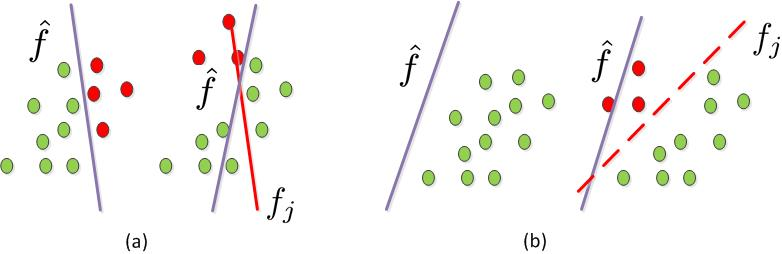
\includegraphics[scale = .6]{fig/domain.jpg}\\
  \caption{(a) Conventional adaptation method fail to find good initialization for the new category from source domain. (b) The parameters from $\hat{f}$ are more adaptive for the new categories.}
  \label{fig:wm}
\end{figure*}
\subsection{Experiment results}

\begin{figure*}
  \centering
  \subfigure{
    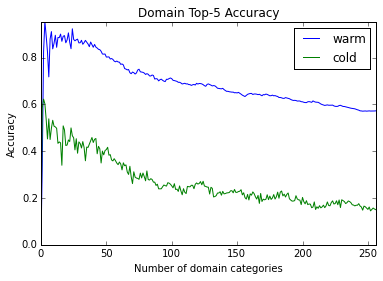
\includegraphics[width=0.4\textwidth]{fig/warm.png}\label{fig:wam_a}
}
\subfigure{
    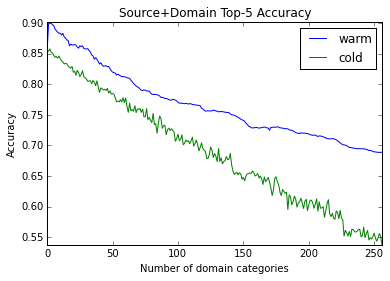
\includegraphics[width=0.4\textwidth]{fig/101_N.png}\label{fig:wam_a}
}
  \centering
\caption{Warm start Vs Cold Start on Top-5 accuracy for limited iterations}
\end{figure*}
